\documentclass[10pt]{article}
\usepackage{geometry}
\geometry{a4paper}
\usepackage{graphicx}
\usepackage{booktabs}
\usepackage{lipsum}
\usepackage{amsmath}
\usepackage{url}
\usepackage{caption}
\usepackage{hyperref}

\usepackage{chngcntr}
\counterwithout{figure}{section}


\title{Time Series Analysis of Propionic Acid-Based Drug Consumption in Veneto, Italy (2016--2023)}
\author{Giuseppe Di Pasquale}
\date{}

\begin{document}
\maketitle
\tableofcontents
\newpage


\begin{abstract}
Effective pharmaceutical resource management requires accurate monitoring systems of consumption patterns to support healthcare planning, supply chain optimization, and policy implementation. This study analyzes consumption patterns of propionic acid-based drugs (ATC code M01AE) in the Veneto region of Italy from 2016 to 2023, aiming to identify seasonal trends, quantify the impact of exogenous factors—particularly COVID-19 lockdown periods, and develop reliable forecasting models for future consumption prediction. The study utilizes monthly dispensing data published by AIFA, applying multiple time series modeling techniques including SARIMA models, ARIMAX with exogenous variables, and Facebook's Prophet algorithm. The analysis reveals consistent seasonal patterns with recurring peaks in January, May, and October, and significant disruption during COVID-19 lockdown periods (April-May 2020). Comparative performance evaluation demonstrates that the ARIMAX model provides superior predictive accuracy on test data, while Prophet shows better fit for training data, suggesting potential overfitting issues. The incorporation of COVID-19 intervention variables significantly improves forecasting accuracy across all tested models. Results indicate consumption stabilization at levels lower than the pre-pandemic period, maintaining characteristic seasonality but with reduced amplitudes. Forecasts for 2024 confirm this trend, projecting monthly volumes between 30,000-40,000 packages with persistence of historical seasonal patterns. These findings provide methodological insights for time series analysis in pharmaceutical contexts and demonstrate the importance of incorporating external shock variables in forecasting models. The developed framework can be extended to analyze other pharmaceutical categories, particularly those influenced by large-scale healthcare disruptions. The study contributes to the growing body of literature examining the long-term impacts of pandemic-related healthcare system changes on pharmaceutical consumption patterns.
\end{abstract}


\section{Introduction}
\label{sec:introduction}

\subsection{The Dataset}
This research utilizes public pharmaceutical consumption data published by the Italian Medicines Agency (AIFA) through their transparency platform. The dataset comprises monthly records of propionic acid-derived medications (ATC code M01AE) dispensed in the Veneto region of Italy between January 2016 and December 2023. These non-steroidal anti-inflammatory drugs (NSAIDs) include widely prescribed medications such as ibuprofen, naproxen, and ketoprofen. The primary variable of interest is the monthly count of drug packages dispensed through both conventional and direct procurement channels.

The time series data spans 96 consecutive months, providing a comprehensive view of consumption patterns before, during, and after significant healthcare events, most notably the COVID-19 pandemic. The dataset does not contain demographic variables or other healthcare indicators, but external events such as the COVID-19 lockdown periods (particularly April-May 2020) have been incorporated as exogenous variables in specific models to assess their impact on consumption patterns.

\subsection{Preprocessing and Data Cleaning}

\subsubsection{Data Description}
The time series data was collated from multiple annual datasets published by AIFA spanning 2016 to 2023. Raw data included region-specific records across all pharmaceutical categories, which were filtered to isolate records specific to the Veneto region and the ATC4 code M01AE (propionic acid derivatives). The number of packages dispensed through both conventional channels and direct procurement were aggregated to obtain the total monthly consumption. 


 We can then plot the series to make some
preliminary observations.

\begin{figure}[ht]
\centering
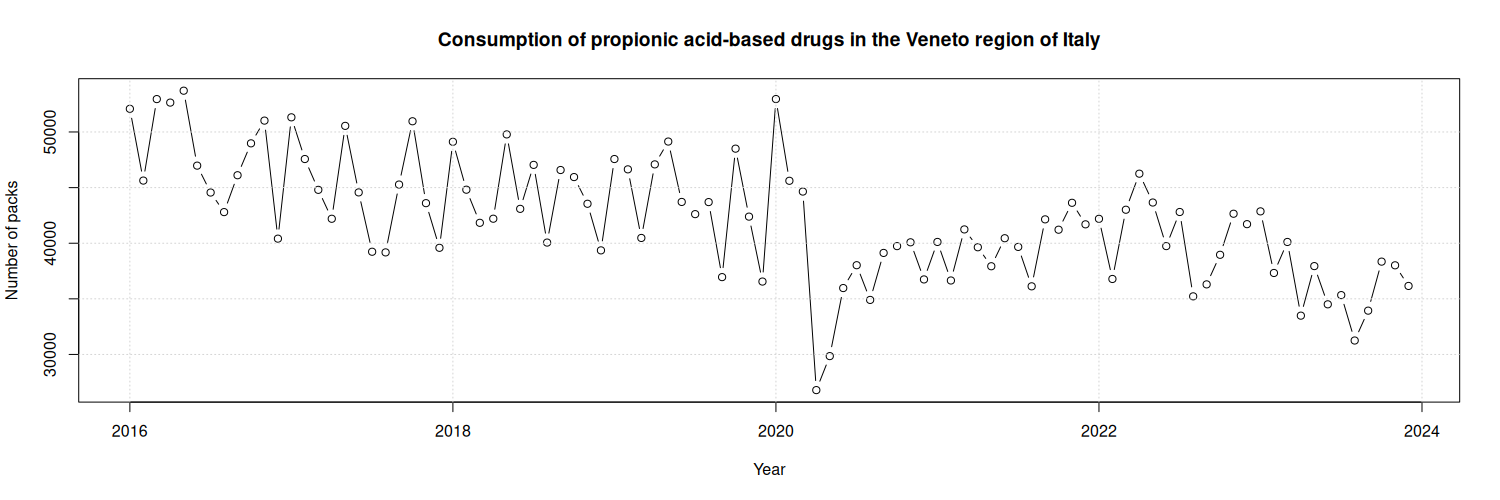
\includegraphics[width=1\textwidth]{Rplot.png}
\caption{Time series of number of packs sold in Veneto throughtout 2016 - 2023.}
\label{fig:data_plot}
\end{figure}

Figure~\ref{fig:data_plot} illustrates the monthly consumption of propionic acid-based drugs in the Veneto region of Italy from 2016 to 2023. A gradual decreasing trend is observable from 2016 through 2019, suggesting a potential long-term reduction in the use of these drugs during that period.

A sharp deviation appears in early 2020, with significant outliers in January, April, and May. These fluctuations coincide with the initial outbreak and subsequent lockdowns related to the COVID-19 pandemic, officially declared in March 2020. The spike in January followed by a steep drop in April and May likely reflects pre-lockdown stockpiling behavior and reduced access to healthcare services during the lockdown period.

Post-2020, the time series stabilizes at a lower consumption level compared to the pre-pandemic years, exhibiting a modest U-shaped or quadratic trend. This may indicate a partial recovery in drug consumption patterns after the initial pandemic shock, albeit without returning to pre-2020 levels, potentially reflecting lasting changes in prescription practices, patient behavior, or healthcare access.

\subsubsection{Time Series Characteristics}

To investigate the temporal structure of propionic acid derivative consumption, we begin by examining the autocorrelation function (ACF) and partial autocorrelation function (PACF) shown in Figure~\ref{fig:acf_pacf_data}. These functions reveal the extent and structure of serial dependence in the time series.

\begin{figure}[ht]
\centering
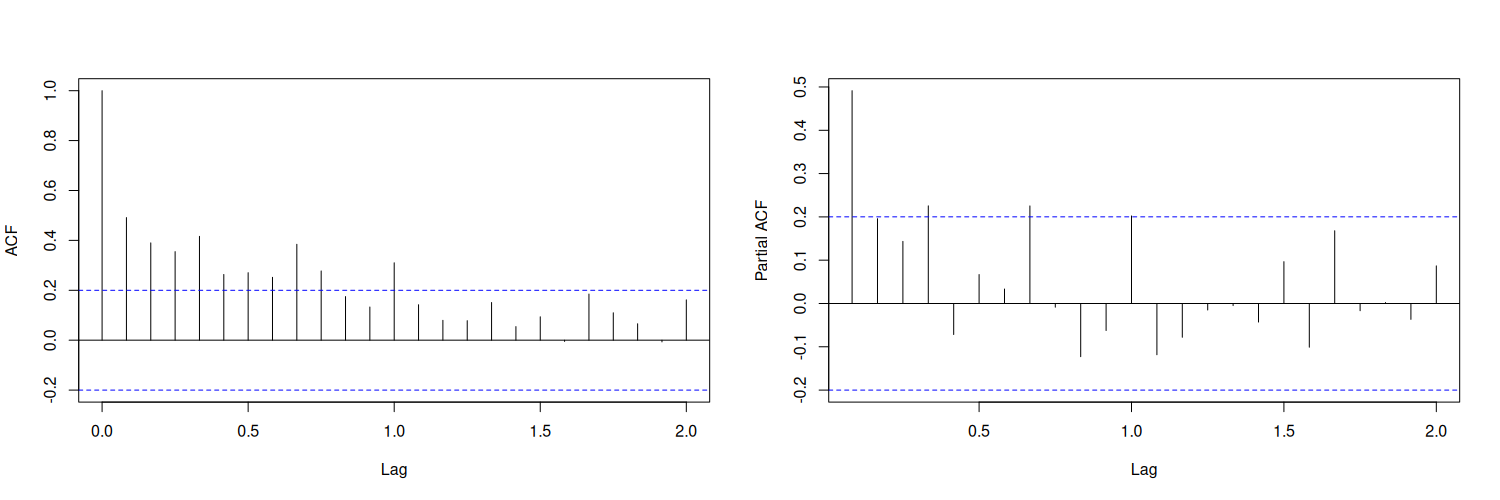
\includegraphics[width=1\textwidth]{Rplot01.png}
\caption{ACF and PACF on the original time series.}
\label{fig:acf_pacf_data}
\end{figure}

The ACF reveals a pronounced spike at lag 0, an expected artifact of self-correlation, followed by a gradual tapering of correlation values as the lag increases. Most of these autocorrelation values lie comfortably within the confidence bounds (indicated by the blue dashed lines), suggesting that, after differencing, the series displays relatively weak serial dependencies. In simpler terms, once we account for past behavior, little structure remains to suggest persistent memory.

The PACF, on the other hand, uncovers a more intricate story. It highlights statistically significant partial autocorrelations at several lags, most notably around lags 0, 0.3, and approximately 1.0. These findings hint at the presence of autoregressive (AR) components in the data: signals that the consumption in a given month may be directly influenced by the preceding month or two. This invites the consideration of AR models, or potentially seasonal ARIMA variants, in forecasting tasks.

\begin{figure}[ht]
\centering
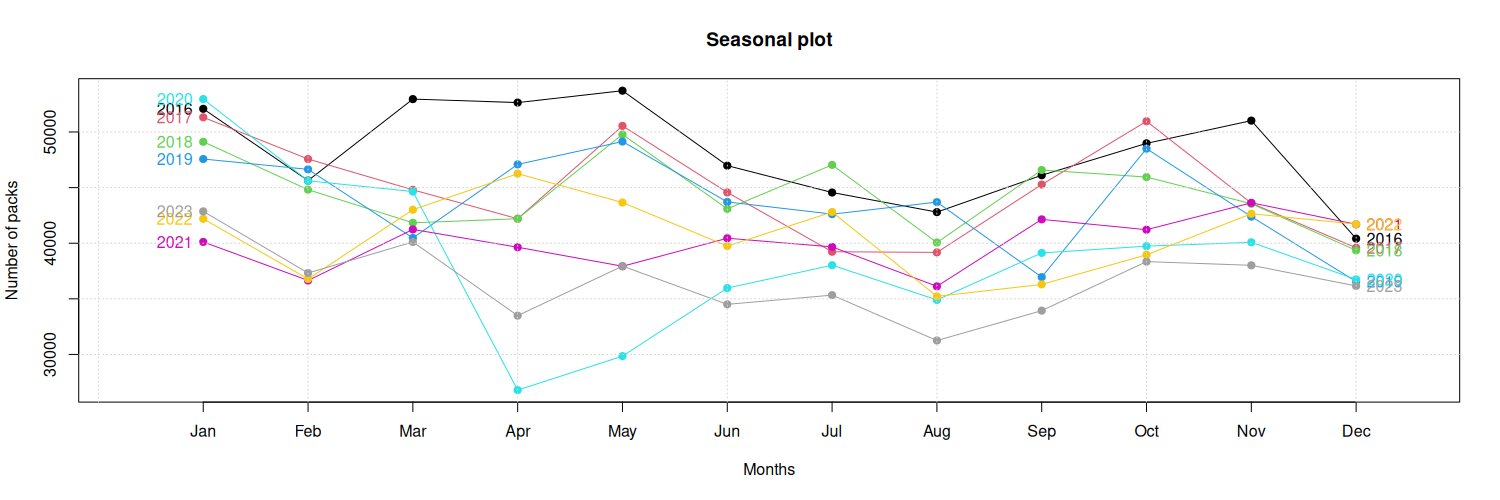
\includegraphics[width=1\textwidth]{Rplot02.png}
\caption{Seasonal mounthly plot, period 2016 - 2023.}
\label{fig:seasonal_data}
\end{figure}

Figure~\ref{fig:seasonal_data} offers a seasonal lens through which we observe the rhythm of consumption throughout the years (2016--2023). This plot overlays monthly values for each year, allowing us to visually extract recurring motifs and deviations in usage patterns.

Three compelling patterns emerge:

\begin{itemize}
    \item \textbf{Seasonal Peaks:} Consumption consistently surges in January, May, and October. The January spike likely reflects a reset in annual prescriptions, while May and October may coincide with seasonal flare-ups of inflammatory conditions.
    
    \item \textbf{Pandemic Disruption:} A striking deviation appears in April 2020, where usage afalls, a signature of the COVID-19 pandemic's disruption. The timing coincides with the onset of stringent public health restrictions that drastically altered healthcare access and behavior.
    
    \item \textbf{Shifting Baselines:} The years 2016 and 2017 show elevated consumption levels compared to later years, pointing to a gradual downward trend preceding the pandemic. Meanwhile, 2022 and 2023 exhibit more subdued seasonal oscillations, possibly signaling a new post-pandemic equilibrium.
\end{itemize}

\subsubsection{Stationarity Assessment}

Stationarity is a fundamental assumption for classical time series modeling and requires thorough evaluation. The rapid decay observed in the ACF suggests that, after differencing, the series may lack persistent autocorrelation—an encouraging sign for stationarity. However, the seasonal decomposition in Figure~\ref{fig:seasonal_data} also reveals structured seasonal cycles and a long‑term trend, both of which violate strict stationarity.

Preliminary visual inspection indicates that achieving stationarity likely requires two transformations:
\begin{enumerate}
  \item \textbf{Seasonal Differencing:} To remove periodic fluctuations.
  \item \textbf{First‑Order Differencing:} To eliminate linear trends.
\end{enumerate}

After these transformations, the series should meet the conditions for applying ARIMA or SARIMA models, which can effectively capture the remaining structure for accurate forecasting.



\subsubsection{Anomaly Detection}

To identify months in which consumption deviates significantly from its expected long‐term trajectory, we first fit a linear trend to the 2016–2019 baseline period (using $n=48$ observations) and assume that the residuals around this trend follow a Student’s $t$‐distribution. 

\begin{figure}[ht]
\centering
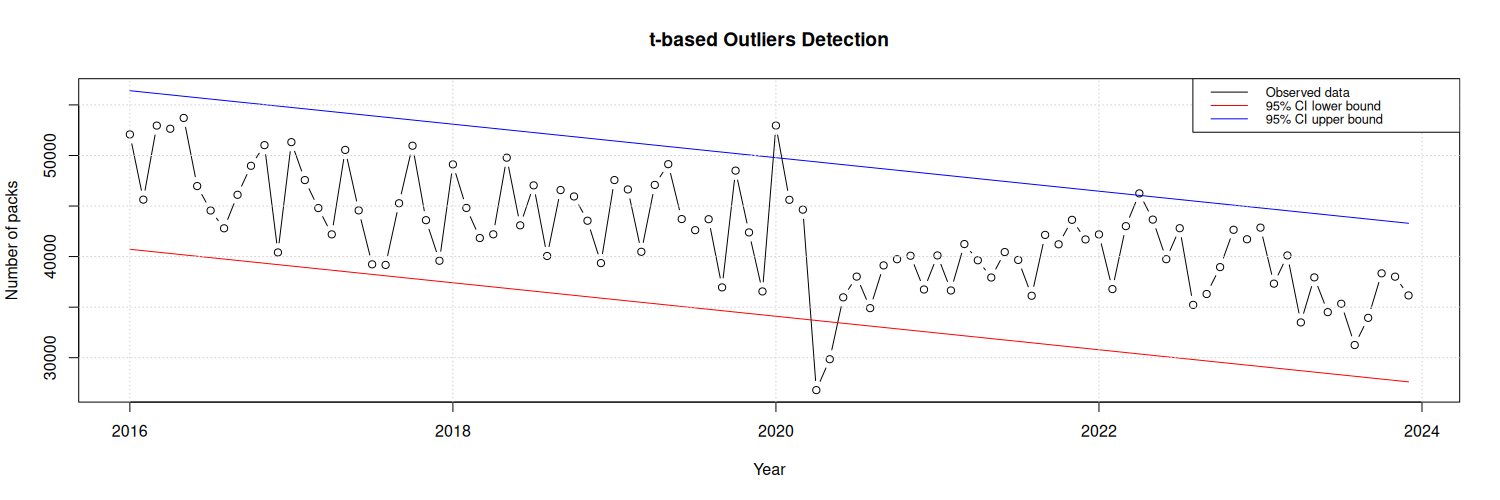
\includegraphics[width=\textwidth]{Rplot03.png}
\caption{Observed monthly consumption (black circles and line) with 95\% $t$‐based confidence bounds around the 2016–2019 trend (red lower bound, blue upper bound).  Points outside the shaded region are classified as anomalies.}
\label{fig:anomaly_detection}
\end{figure}

Figure~\ref{fig:anomaly_detection} overlays the fitted 2016–2019 trend with its 95\% $t$‐based confidence interval and highlights those months whose observed values lie beyond these limits.  Three key events are apparent:

\begin{itemize}
  \item \textbf{January 2020 (COVID‑19 Awareness):} Although still within the expected range, January 2020 marks the initial period of heightened awareness about COVID‑19.  Consumption remains on‐trend here, but it sets the stage for the subsequent disruption.
  \item \textbf{April 2020 (Pandemic Disruption):} Consumption in April 2020 falls well below the lower confidence bound, reflecting the abrupt impact of lockdowns and restricted healthcare access.  This drop is visibly anomalous against the pre‐pandemic trajectory.
  \item \textbf{May 2020:} In May 2020, toward the end of the lockdown, a "catch-up" effect begins to emerge. However, usage levels remain outside the confidence interval and are consequently classified as an anomaly.
  \item \textbf{May 2022 Outlier (Excluded):} Although May 2022 briefly appears outside the 95\% bounds—likely driven by a localized supply‐chain issue—we do not consider it a primary anomaly for this analysis and omit further discussion.
\end{itemize}

By employing a $t$‐distribution framework appropriate for $n=48$ (2016–2019), we accommodate heavier tails than a normal approximation and obtain more reliable confidence bounds.  Any future monthly observation that falls outside these intervals warrants further investigation for external shocks (e.g., policy shifts, seasonal outbreaks, or regulatory changes).  In particular, the early‐2020 anomalies correspond directly to COVID‑19’s disruption and recovery phases, underscoring the value of this method in detecting unanticipated events.  




\section{Model Testing}

We developed and tested multiple forecasting models to capture the complex patterns in propionic acid-based drug consumption. The data was split into training (January 2016 to December 2022) and testing (January 2023 to December 2023) sets to evaluate predictive performance.
\subsection{ARIMA Models}

\subsubsection{Base SARIMA Model}

To model the monthly consumption series without external regressors, we employed the \texttt{auto.arima()} function in R, which performs a stepwise search to minimize the Akaike Information Criterion (AIC).  The selected model was $\text{ARIMA}(0,1,1)(1,0,0)_{12}$.

Figure~\ref{fig:sarima} displays the residual diagnostics for this base SARIMA model.  The top panel shows the residual series over time, while the bottom two panels present the sample ACF and PACF of the residuals (lags up to 24 months). 

\begin{figure}[ht]
\centering
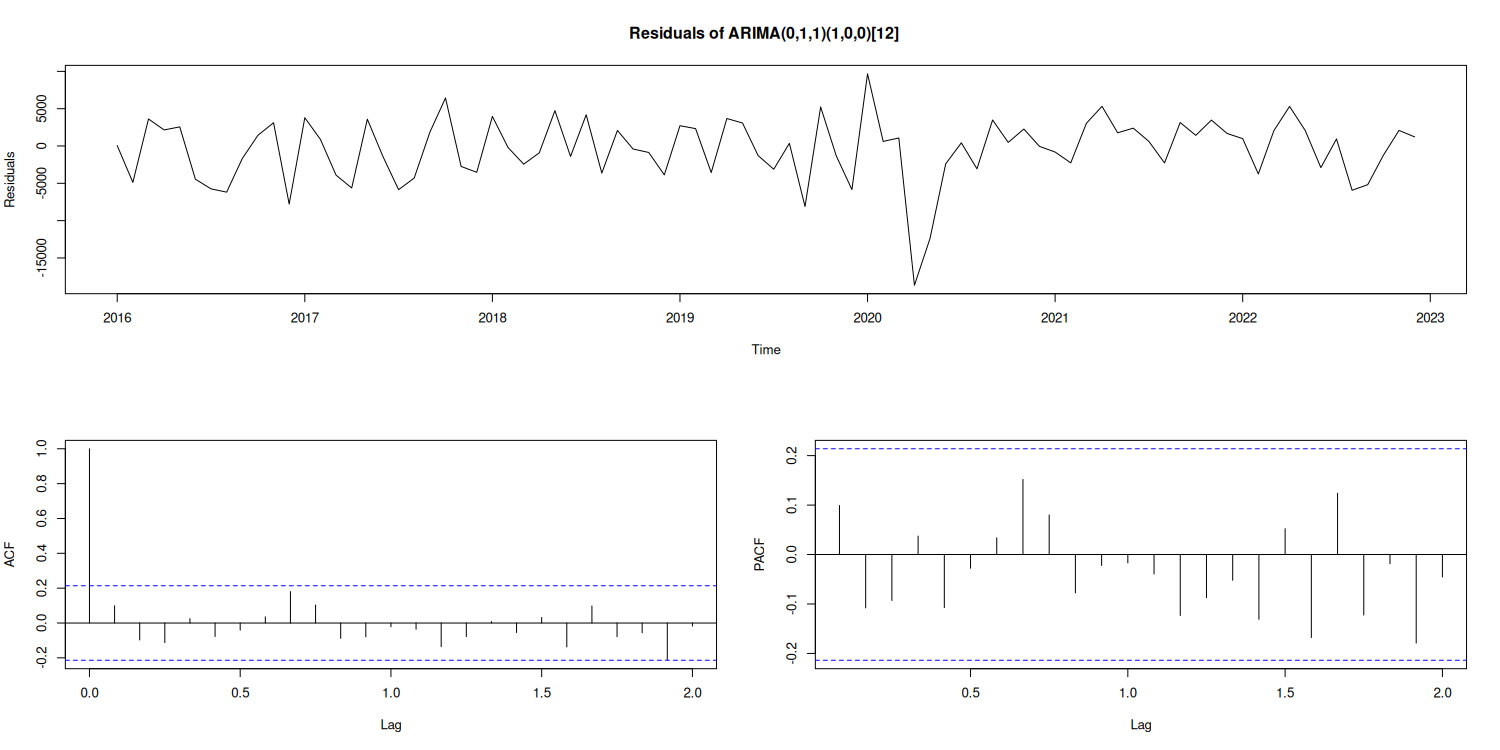
\includegraphics[width=\linewidth]{Rplot04.png}
\caption{Residual diagnostics for $\text{ARIMA}(0,1,1)(1,0,0)_{12}$: (top) residual time series; (bottom left) ACF of residuals; (bottom right) PACF of residuals.  Dashed blue lines denote approximate 95\% confidence bounds.}
\label{fig:sarima}
\end{figure}

A close inspection of Figure~\ref{fig:sarima} indicates that:
\begin{itemize}
  \item \textbf{Residual Time Series:} The residuals fluctuate around zero without a clear trend or persistent structure.  Although a large negative spike appears in early 2020, consistent with the April 2020 pandemic‐related disruption, no systematic pattern remains thereafter.
  \item \textbf{ACF of Residuals:} All autocorrelation coefficients lie within the 95\% confidence bounds (dashed lines), suggesting that the model has successfully removed serial dependence.  In particular, there are no significant spikes at seasonal lags (e.g., 12 or 24).
  \item \textbf{PACF of Residuals:} Similarly, the sample partial autocorrelations do not exceed their confidence limits, confirming the absence of unmodeled AR components.  Minor fluctuations at intermediate lags are within expected random variation.
\end{itemize}

In addition to these visual checks, the Ljung–Box test (up to lag 24) yields $p>0.05$, providing no evidence of remaining autocorrelation.  


\subsubsection{SARIMA with COVID–19 Intervention Variables}

To account for the sharp disruption in consumption caused by the COVID–19 pandemic, we extended the base SARIMA model by incorporating intervention dummies for the key months affected. Specifically, we included binary indicators for:
\begin{itemize}
    \item \textbf{Awareness} in January 2020, marking the first global alerts about the outbreak;
    \item \textbf{Lockdown} in April and May 2020, corresponding to the period of peak restrictions.
\end{itemize}

The resulting model is an ARIMA(0,1,1)(1,0,1)\textsubscript{12} with exogenous regressors.

Both intervention terms were found to be statistically significant ($p < 0.01$), indicating that the model successfully captures the large deviations in consumption associated with the early stages of the pandemic. In particular, the Awareness coefficient $\beta_1$ captures the anticipatory behavioral response in January, while $\beta_2$ reflects the sharp drop in April and May.

Figure~\ref{fig:sarima_covid} presents the residual diagnostics for this extended model. As with the base model, residuals show no strong evidence of autocorrelation, and the variance remains stable over time. Notably, the intervention terms effectively absorb the outliers from early 2020, bringing residuals within a comparable range to those seen in the pre-pandemic period.

\begin{figure}[ht]
\centering
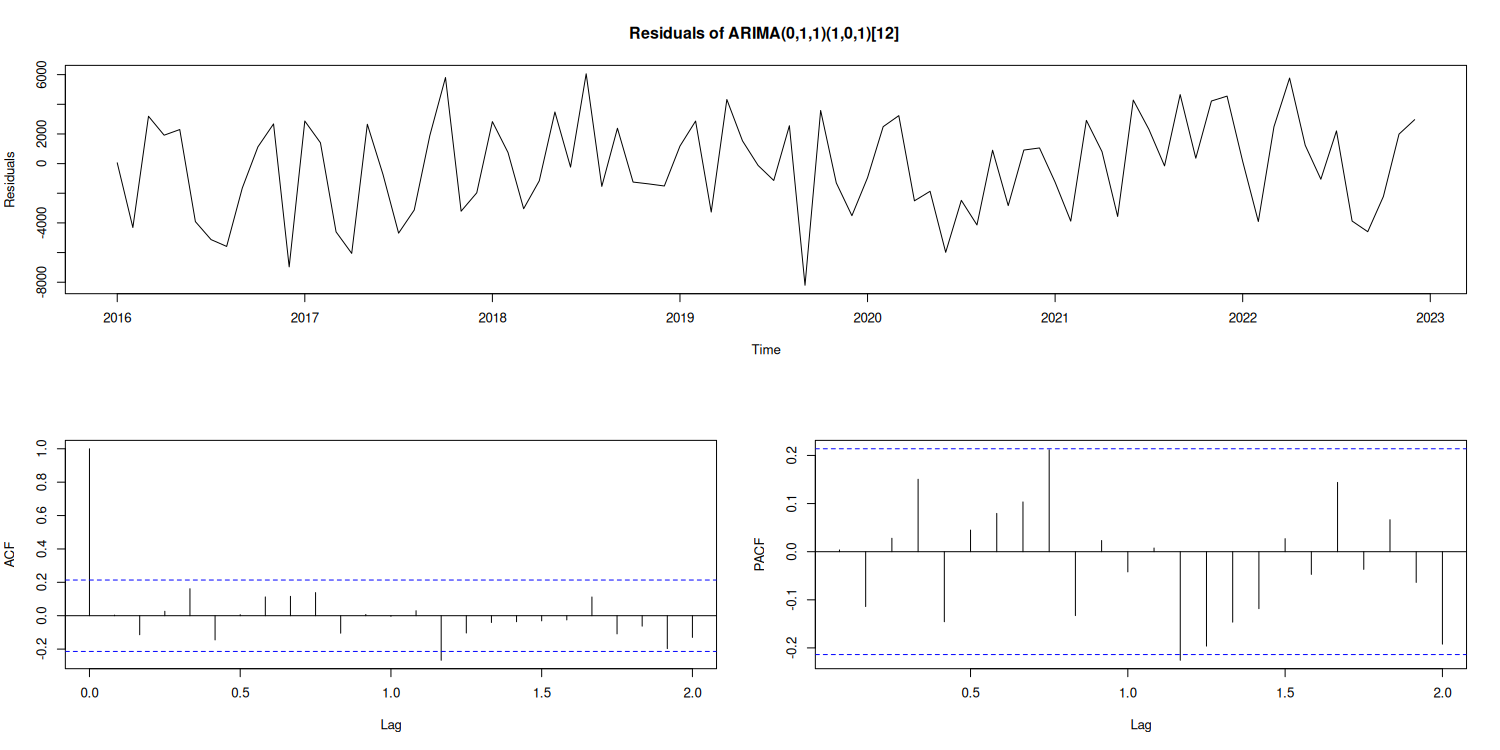
\includegraphics[width=\linewidth]{Rplot05.png}
\caption{Residual diagnostics for ARIMA(0,1,1)\,(1,0,1)\textsubscript{12} with COVID–19 intervention variables: (top) residual time series; (bottom left) ACF of residuals; (bottom right) PACF of residuals. Dashed blue lines indicate approximate 95\% confidence bounds.}
\label{fig:sarima_covid}
\end{figure}

Overall, the addition of COVID–19–specific regressors improves model interpretability and predictive accuracy by explicitly addressing the pandemic's structural break. 


\subsection{ARIMAX Model}
Building on the previous models, we developed a comprehensive ARIMAX model incorporating both time trend and seasonal components as exogenous variables.

After examining the residuals from this regression, we identified that an $\text{ARIMA}(0,1,1)(0,0,0)_{12}$ model effectively addressed the remaining autocorrelation, confirming that seasonal effects are adequately captured by the regression component, and no additional seasonal structure is needed in the ARIMA errors.

This two-step approach allowed us to explicitly model both deterministic components (trend, seasonality) and stochastic dependencies in the data, providing a robust framework for analyzing the impact of COVID-19 on pharmaceutical consumption patterns in the region. Figure~\ref{fig:arimax} presents the residual diagnostics for the final model.

\begin{figure}[ht]
\centering
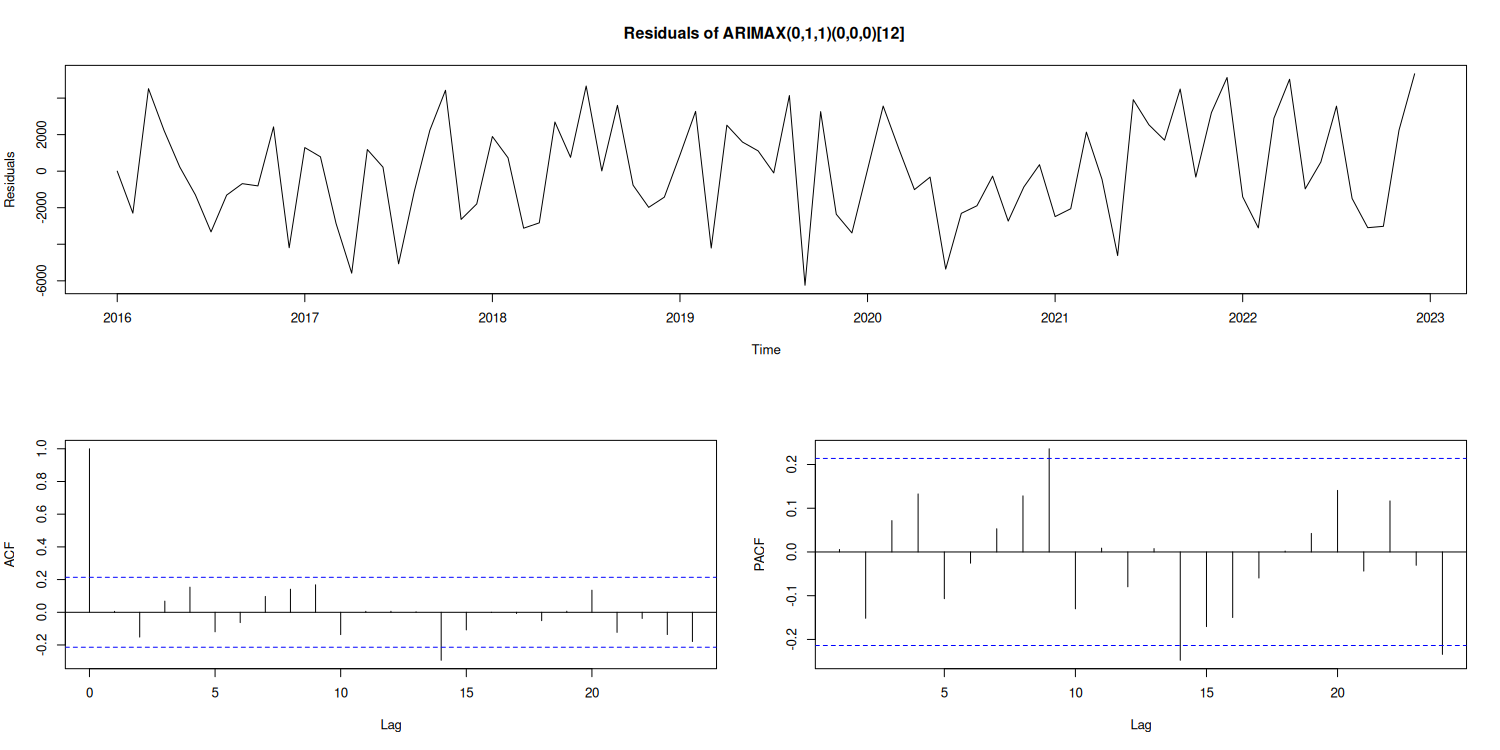
\includegraphics[width=1\linewidth]{Rplot06.png}
\caption{Residual diagnostics for the ARIMAX(0,1,1)(0,0,0)$_{12}$ model: (top) residual time series plot showing homoscedasticity from 2016 to 2023; (bottom left) ACF of residuals showing no significant autocorrelation beyond the confidence bounds; (bottom right) PACF of residuals similarly indicating successful capture of the temporal dependence structure. The dashed blue lines indicate approximate 95\% confidence bounds.}
\label{fig:arimax}
\end{figure}

As evident from Figure~\ref{fig:arimax}, the residuals of our ARIMAX model exhibit the desirable properties of white noise. The time series plot of residuals shows no discernible pattern, and the ACF and PACF plots demonstrate minimal significant autocorrelation, with nearly all lags falling within the 95\% confidence bounds (represented by the dashed blue lines). This indicates that our model has successfully captured the underlying dynamics of propionic acid-base drug consumption in Veneto.

\subsection{Prophet Model}
As an alternative methodological approach, we implemented Facebook's Prophet algorithm, which is specifically designed for forecasting time series with strong seasonal effects and historical trends. 

We configured the Prophet model with the following specifications:
\begin{itemize}
    \item Annual seasonality enabled to capture yearly consumption patterns
    \item COVID-19 awareness period (January 2020) incorporated as a change point
    \item Lockdown periods (April-May 2020) included as special events
    \item Daily and weekly seasonality disabled as our data is aggregated monthly
    \item Multiplicative seasonality to account for varying amplitude in seasonal patterns
\end{itemize}

Prophet automatically identified critical changepoints in the series, which aligned closely with the beginning of the COVID-19 pandemic and subsequent recovery phases in Veneto. The flexibility of the Prophet framework allowed us to model complex, non-linear trends that might not be fully captured by traditional ARIMA-based approaches.

\begin{figure}[ht]
\centering
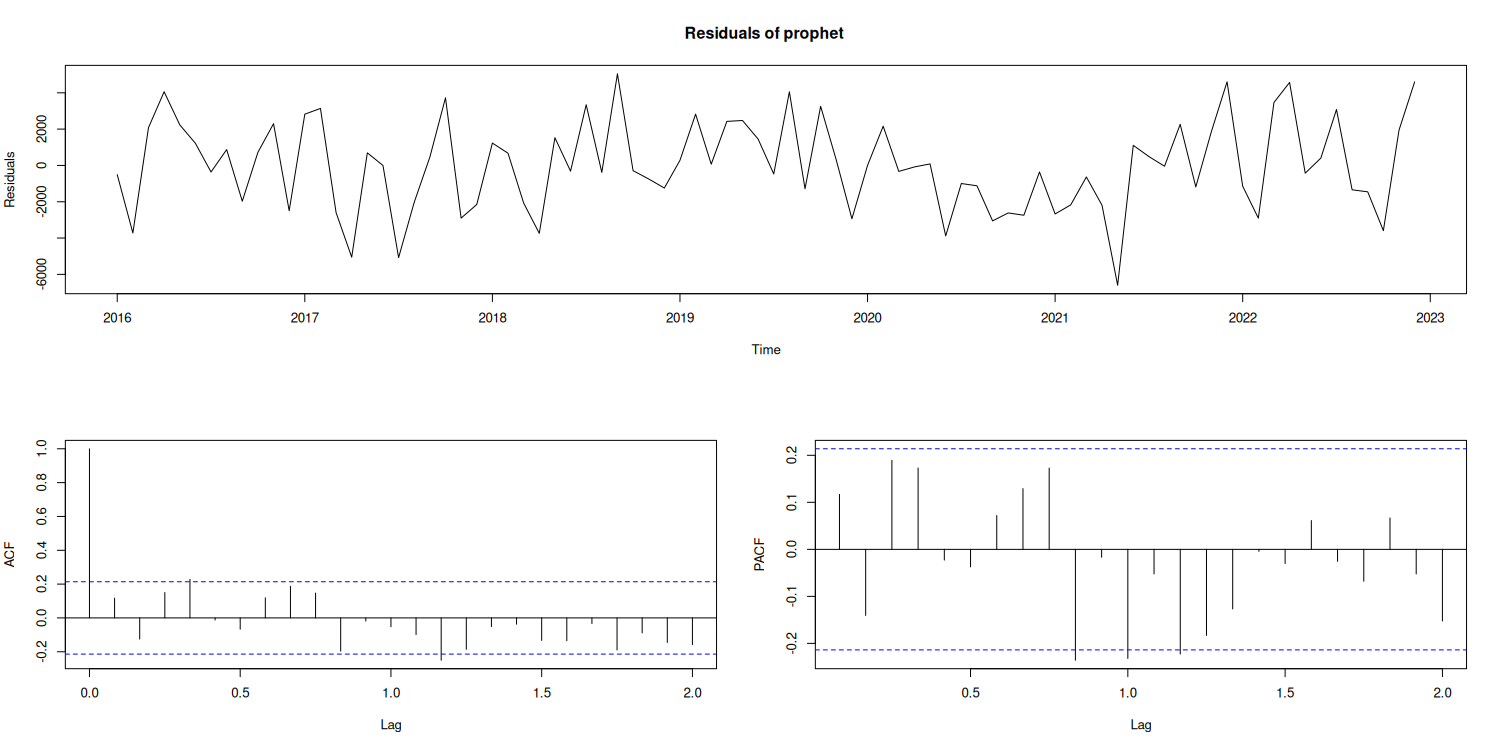
\includegraphics[width=1\linewidth]{Rplot07.png}
\caption{Residual diagnostics for the Prophet model: (top) residual time series showing consistent variance across the observation period; (bottom left) ACF of residuals demonstrating effective capture of temporal dependencies with minimal significant autocorrelation; (bottom right) PACF of residuals showing similar pattern quality. Dashed blue lines indicate approximate 95\% confidence bounds.}
\label{fig:prophet}
\end{figure}

The residual diagnostics presented in Figure~\ref{fig:prophet} demonstrate that the Prophet model effectively captures the temporal dynamics in the data. The residual plot shows a pattern similar to that of the ARIMAX model, with no obvious trends or heteroscedasticity. The ACF and PACF plots similarly indicate minimal significant autocorrelation at most lags, though with slightly different patterns than the ARIMAX model. This suggests that both modeling approaches have merit in analyzing the pharmaceutical consumption data, with potential complementary insights.



\section{Results}

This section presents a comprehensive evaluation of the forecasting models developed to predict the number of packs over the time period from 2016 to 2023. Four distinct time series forecasting approaches were implemented: SARIMA, SARIMA with COVID adjustment, ARIMAX, and Prophet. The evaluation process employs a two-pronged approach to determine the optimal model for the given dataset.

First, we conduct a visual analysis to qualitatively assess how accurately each model captures the historical patterns in the training data (2016-2022) and predicts future values in the test data (2023). This visual inspection allows us to identify each model's ability to respond to seasonal fluctuations, structural changes, and anomalies such as the COVID-19 disruption.

Following the visual assessment, we will present a quantitative metrics comparison using standard performance indicators such as Mean Absolute Error (MAE), Root Mean Square Error (RMSE), and Mean Absolute Percentage Error (MAPE). These metrics provide objective measures of forecast accuracy and will complement the visual analysis to support a data-driven selection of the most appropriate forecasting model for this particular time series.


\subsection{Visual Comparison}

This section analyzes the performance of four time series forecasting models (SARIMA, SARIMA with COVID adjustment, ARIMAX, and Prophet) on both training data (2016-2022) and test data (2023).

\subsubsection{Fitted Values on Training Data (2016-2022)}
Figure~\ref{fig:fitted_train} provides valuable insights into the comparative behavior of the forecasting models.

All models effectively capture the underlying seasonal patterns present in the data. Among them, the Prophet model stands out for its high sensitivity to short-term fluctuations, frequently realigning its trajectory to closely follow observed data points. While this responsiveness can be advantageous in dynamic settings, it also suggests a tendency toward overfitting, as the model prioritizes immediate alignment over long-term stability.

In contrast, both SARIMA variants produce smoother forecasts, effectively capturing medium-term trends while filtering out transient noise. Notably, the SARIMA model with a COVID adjustment offers a marginal improvement over the standard version, particularly in its handling of the 2020 anomaly and subsequent recovery period.

The ARIMAX model exhibits a balanced behavior between the extremes of Prophet’s high reactivity and SARIMA’s stability. It effectively captures major structural shifts in the data while maintaining a more tempered response to short-term variability.

During the pre-pandemic period (2016–2019), all models demonstrate comparable accuracy, with no single approach consistently outperforming the others across all segments.

Following 2020, the data undergoes a subtle regime shift, characterized by slightly lower average values and dampened fluctuations. While this change poses a modeling challenge, all models adjust reasonably well to the new dynamics, albeit with some variance in adaptability.


\begin{figure}[ht]
\centering
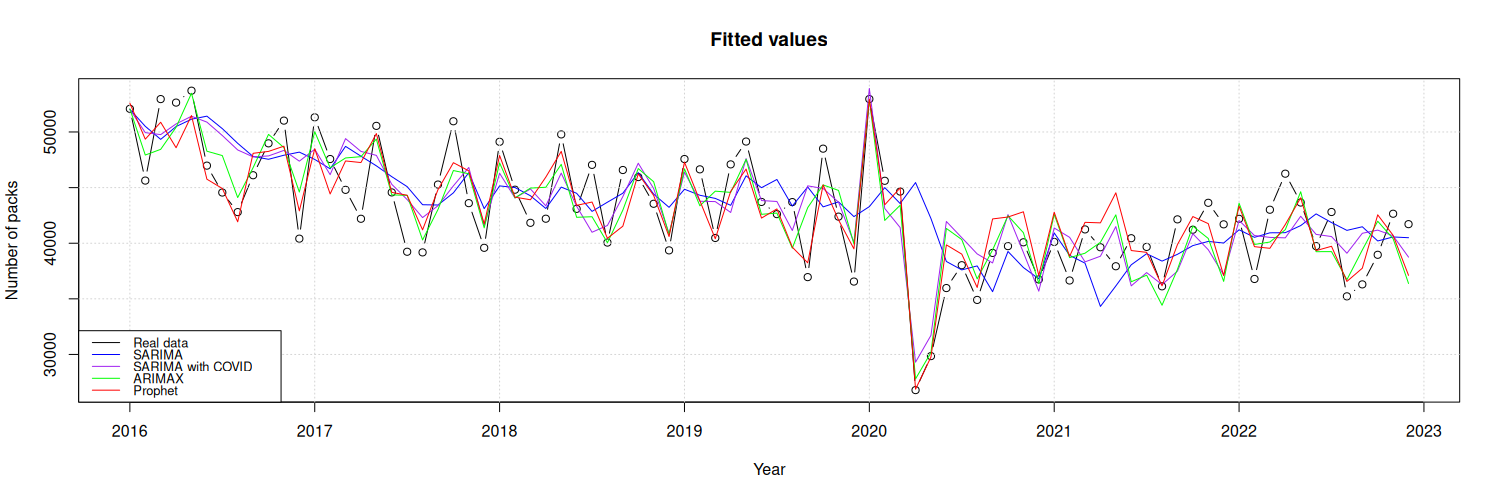
\includegraphics[width=1\linewidth]{Rplot08.png}
\caption{Fitted values on train data.}
\label{fig:fitted_train}
\end{figure}


\subsubsection{Forecasted Values on Test Data (2023)}

Figure~\ref{fig:forcasted_test} highlights substantial discrepancies between model predictions and observed values during the test period.

The most striking observation is that all models consistently overestimate actual values throughout 2023, typically by 2,000-6,000 units. This systematic bias indicates that none of the approaches successfully captured either a fundamental shift in the underlying process or new external factors affecting pack numbers.

Model forecasts demonstrate markedly different behavior than the actual data in terms of volatility. While the observed values (black line) show sharp fluctuations between adjacent months, particularly the severe April and August dip to approximately 8,000 and 6,000 units, all model predictions present smoother trajectories. This suggests limitations in capturing the true variability of the process when projecting forward.

Despite their different methodological foundations, the models produce relatively similar forecast patterns, with Prophet showing slightly more pronounced seasonal variations than the SARIMA variants. This convergence in predictions, despite divergent approaches, highlights the challenge of forecasting when the system undergoes changes not reflected in historical patterns.

The models correctly anticipate the general seasonal low point in August, demonstrating some success in capturing recurring annual patterns. However, they fail to predict the magnitude of this dip and the subsequent sharp recovery through October. This indicates that while the models understand basic seasonality, they struggle with projecting changing amplitudes in these patterns.

The forecast accuracy comparison reveals an important methodological insight: good performance on training data does not necessarily translate to accurate predictions. The Prophet model's tight tracking of historical data points did not yield superior forecasts, suggesting that its apparent advantage in the training period may indeed represent overfitting rather than superior pattern recognition.

The SARIMA variants, despite their smoother and potentially less impressive fit to historical fluctuations, produce forecasts of comparable quality to the more complex models. This reinforces the principle of parsimony in time series forecasting—simpler models often demonstrate similar or better generalization to new data compared to more elaborate approaches.

\begin{figure}[ht]
\centering
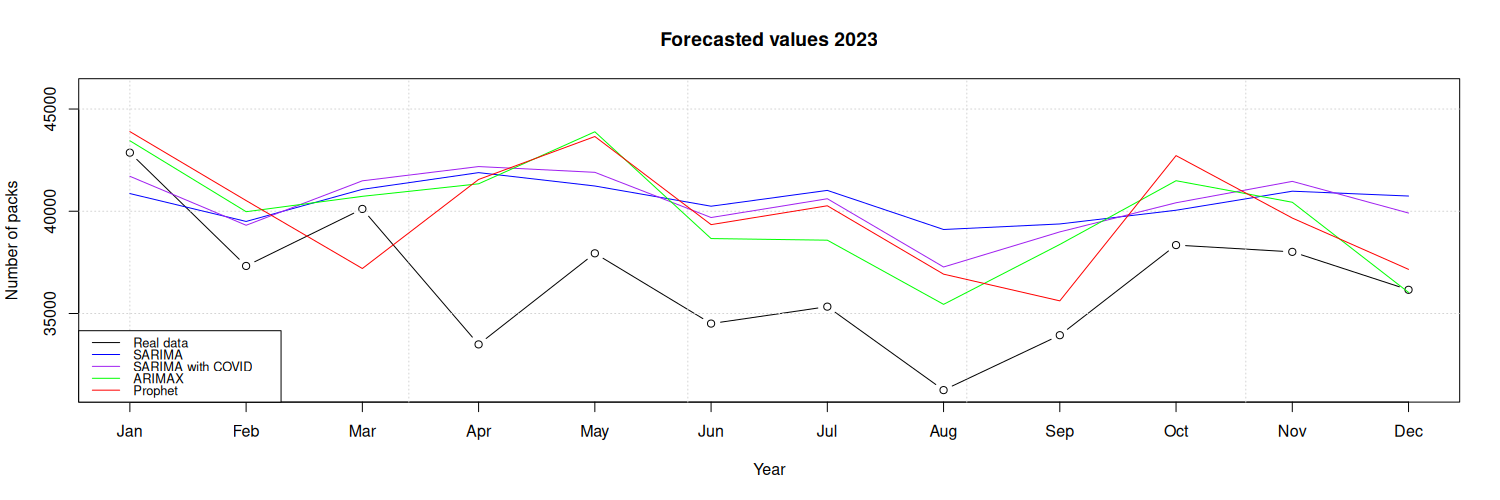
\includegraphics[width=1\linewidth]{Rplot09.png}
\caption{Forcasted values for test data.}
\label{fig:forcasted_test}
\end{figure}



\subsection{Performance Metrics Analysis}

\subsubsection{Evaluation Framework}
We evaluated four time series forecasting models using multiple performance metrics on both training (2016-2022) and testing (2023) data: Mean Error (ME), Mean Absolute Error (MAE), Root Mean Square Error (RMSE), Mean Percentage Error (MPE), and Mean Absolute Percentage Error (MAPE). MAE and RMSE were prioritized due to their robustness and intuitive interpretation.

\begin{table}[ht]
\centering
\begin{tabular}{lrrrrr}
    \hline
    Models & ME & MAE & RMSE & MPE & MAPE \\ 
    \hline
    SARIMA & -457.99 & 3252.75 & 4280.02 & -2.02 & 8.05 \\ 
    SARIMA with COVID & -213.08 & 2759.44 & 3255.21 & -0.99 & 6.57 \\ 
    ARIMAX & -18.02 & 2330.73 & 2806.63 & 0.32 & 5.52 \\ 
    Prophet & -0.05 & 1998.36 & 2490.38 & 0.34 & 4.67 \\ 
    \hline
\end{tabular}
\caption{Performance Metrics on Train Set (2016-2022)}
\label{train_metrics}
\end{table}

\begin{table}[ht]
\centering
\begin{tabular}{lrrrrr}
    \hline
    Models & ME & MAE & RMSE & MPE & MAPE \\ 
    \hline
    SARIMA & 3900.22 & 4233.31 & 4833.15 & 11.34 & 12.12 \\ 
    SARIMA with COVID & 3806.13 & 3998.55 & 4520.92 & 10.95 & 11.40 \\ 
    ARIMAX & 3261.18 & 3282.58 & 3933.78 & 9.26 & 9.32 \\ 
    Prophet & 3270.13 & 3755.62 & 4311.28 & 9.37 & 10.58 \\ 
    \hline
\end{tabular}
\caption{Performance Metrics on Test Set (2023)}
\label{test_metrics}
\end{table}

\subsubsection{Key Findings}
The tables reveal critical insights into model performance:

\textbf{Training Performance:} Prophet achieved the best in-sample fit, followed by ARIMAX, COVID-adjusted SARIMA, and standard SARIMA. Prophet's superior training metrics aligned with its observed high sensitivity to historical fluctuations.

\textbf{Testing Performance:} All models systematically overestimated 2023 values, with ARIMAX demonstrating the best test performance (lowest MAE: 3282.58, RMSE: 3933.78). Prophet's performance advantage vanished in the test period, with its MAE increasing by 88\% compared to training.

\textbf{Performance Comparison:} The superior in-sample fit did not translate to better forecasting capability. ARIMAX maintained the optimal balance between fit and prediction accuracy, while Prophet showed signs of overfitting. COVID-adjusted SARIMA consistently outperformed the standard version.

\subsubsection{Conclusion}
The contrast between in-sample and out-of-sample performance demonstrates the critical importance of validation testing. The universal overestimation in 2023 suggests new factors affecting package volumes not captured in historical patterns. ARIMAX emerges as the most effective model, balancing sophistication with practical utility while providing superior forecasting accuracy.


\section{Forecasting}

After comprehensive model evaluation, we retrained all models on the complete dataset (2016-2023) to generate forecasts for 2024. The integration of 2023 observations—where all models previously overestimated actual values—provided critical calibration for improving predictive accuracy.

\begin{figure}[ht]
\centering
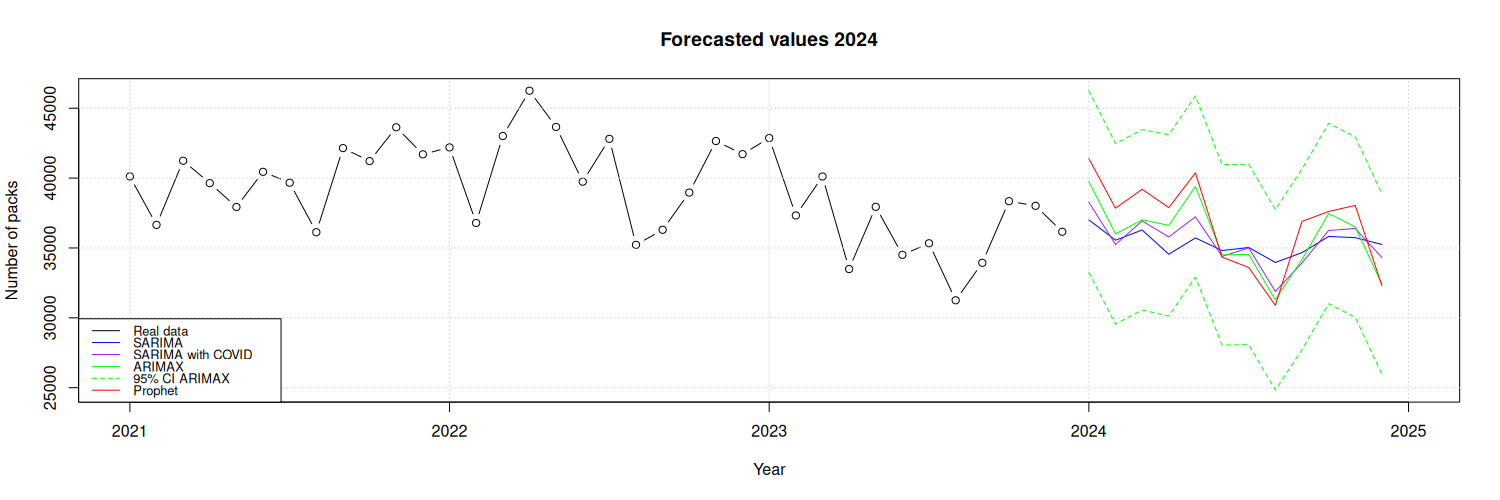
\includegraphics[width=1\linewidth]{Rplot10.png}
\caption{Forecasted values for 2024 based on the complete 2016-2023 dataset, showing consensus on seasonal patterns despite variations in projected volume levels.}
\label{fig:forecast_2024}
\end{figure}

Figure~\ref{fig:forecast_2024} reveals notable convergence in the seasonal trajectory across all models, with projected monthly package volumes between 30,000-40,000 units. All forecasts anticipate a characteristic dip in August-September followed by fourth-quarter recovery, consistent with historical patterns. However, the models diverge in their baseline projections: Prophet consistently forecasts higher volumes, SARIMA variants project lower ranges, and ARIMAX produces intermediate estimates that balance recent trends with longer-term patterns.

The ARIMAX model's 95\% confidence interval (dotted green lines) illustrates the inherent uncertainty in these forecasts, with a prediction range expanding to approximately 15,000 units by late 2024. This progressive widening reflects the increasing difficulty of long-term projections, particularly for a series that has undergone structural shifts during the COVID-19 pandemic and subsequent healthcare adjustments.

Based on comparative performance metrics and theoretical considerations, we recommend adopting the ARIMAX forecast as the primary planning baseline while utilizing its confidence intervals for contingency thresholds. The implementation strategy should include: (1) monthly forecast updates as new data becomes available; (2) systematic monitoring of accuracy metrics to detect potential emerging biases; and (3) cross-functional input to identify new external factors that might influence consumption patterns beyond historical precedents.

The forecast suggests that propionic acid derivative consumption in Veneto will stabilize at levels lower than pre-pandemic observations, reflecting potentially lasting changes in prescribing practices or healthcare utilization patterns. The pronounced seasonality remains a reliable operational planning guide despite these structural shifts.

\section{Conclusions}

This study analyzed the consumption patterns of propionic acid-based drugs in the Veneto region of Italy from 2016 to 2023, with particular attention to pandemic-related disruptions and the development of reliable forecasting methodologies for pharmaceutical planning. Several key findings emerge from our analysis:

\begin{itemize}
    \item The time series demonstrated distinct seasonal patterns with consistent peaks in January, May, and October, and predictable troughs in August-September. This seasonality persisted throughout the observation period despite overall consumption levels declining gradually from 2016 through 2019, followed by a more pronounced reduction during and after the COVID-19 pandemic.
    \item Anomaly detection confirmed significant outliers during the initial pandemic period (April-May 2020), representing substantial deviations from expected values based on pre-pandemic trends. These outliers reflected the acute impact of lockdown measures on healthcare accessibility and patient behavior. Subsequent stabilization occurred at lower average consumption levels compared to pre-pandemic years, suggesting a potential structural shift in prescription patterns or healthcare utilization.
    \item Our comparative model evaluation revealed that ARIMAX delivered superior predictive performance on test data despite Prophet showing better fit for training observations. This highlights the critical distinction between in-sample fit and forecasting capability, with over-parameterized models potentially sacrificing generalizability for historical precision. The explicit modeling of COVID-19 intervention variables significantly improved forecast accuracy across all model types.
    \item Our 2024 forecasts project stabilized consumption patterns with preserved seasonality but at generally lower volumes than pre-pandemic levels. The convergence of projections across disparate modeling approaches increases confidence in the forecasted seasonal patterns, while the variations in baseline estimates underscore the inherent uncertainty in long-term predictions for systems that have experienced structural shifts.
\end{itemize}

These results provide useful insights into the consumption dynamics of propionic acid-based medications. The modeling approach developed in this project is flexible and can be applied to other pharmaceutical categories, especially those influenced by large-scale healthcare disruptions. For future work, incorporating additional external factors—such as demographic changes, policy shifts, or trends in alternative treatments, could help improve forecast accuracy and model robustness.


\newpage
\section*{Acknowledgments}
The authors acknowledge the Italian Medicines Agency (AIFA) for providing access to pharmaceutical consumption data through their public transparency platform.

\begin{thebibliography}{1}
\bibitem{(AIFA)} Agenzia Italiana del Farmaco.\\ \textit{Spesa e consumo relativi al flusso della farmaceutica convenzionata e degli acquisti diretti}.\\ \href{https://www.aifa.gov.it/spesa-e-consumo-relativi-al-flusso-della-farmaceutica-convenzionata-e-degli-acquisti-diretti} {https://www.aifa.gov.it/spesa\allowbreak-e\allowbreak-consumo\allowbreak-relativi\allowbreak-al\allowbreak-flusso\allowbreak-della\allowbreak-farmaceutica\allowbreak-convenzionata\allowbreak-e-degli\allowbreak-acquisti\allowbreak-diretti}

\end{thebibliography}



\end{document}
